%%%%%%%%%%%%%%%%%%%%%%%%%%%%%%%%%%%%%%%%%
% University/School Laboratory Report
% LaTeX Template
% Version 3.1 (25/3/14)
%
% This template has been downloaded from:
% http://www.LaTeXTemplates.com
%
% Original author:
% Linux and Unix Users Group at Virginia Tech Wiki 
% (https://vtluug.org/wiki/Example_LaTeX_chem_lab_report)
%
% License:
% CC BY-NC-SA 3.0 (http://creativecommons.org/licenses/by-nc-sa/3.0/)
%
%%%%%%%%%%%%%%%%%%%%%%%%%%%%%%%%%%%%%%%%%

%----------------------------------------------------------------------------------------
%	PACKAGES AND DOCUMENT CONFIGURATIONS
%----------------------------------------------------------------------------------------

\documentclass{article}

\usepackage[version=3]{mhchem} % Package for chemical equation typesetting
%\usepackage{siunitx} % Provides the \SI{}{} and \si{} command for typesetting SI units
\usepackage{graphicx} % Required for the inclusion of images
\usepackage{natbib} % Required to change bibliography style to APA
\usepackage{amsmath} % Required for some math elements 
\usepackage{hyperref}
 \usepackage{pdflscape}
\usepackage[a4paper,margin=0.5in]{geometry}
\setlength\parindent{0pt} % Removes all indentation from paragraphs

\renewcommand{\labelenumi}{\alph{enumi}.} % Make numbering in the enumerate environment by letter rather than number (e.g. section 6)

%\usepackage{times} % Uncomment to use the Times New Roman font

%----------------------------------------------------------------------------------------
%	DOCUMENT INFORMATION
%----------------------------------------------------------------------------------------

\title{Gate Detection} % Title

\author{Philipp \textsc{Duernay}} % Author name

\date{\today} % Date for the report

\begin{document}
\maketitle
% If you wish to include an abstract, uncomment the lines below
% \begin{abstract}
% Abstract text
% \end{abstract}

%----------------------------------------------------------------------------------------
%	SECTION 1
%----------------------------------------------------------------------------------------

\section{Recap}
In the last meeting from 06.06.2018 several next steps were defined:
\begin{itemize}
	\item Investigate coarse to fine approach/ region proposal approach
	\item See if tensorflow-lite actually uses the gpu
\end{itemize}


\section{Darknet}

As it turned out tensorflow-lite does not use the GPU which is probably the reason why it is so much slower than darknet (the yolo framework). Also does darknet use a particular set of processor instructions that allow faster computation.

Good news is I was able to train a smaller version of yolo on the gate data. It is relatively simple to change the hyperparameters of yolo within darknet. Soon I can report the inference time for this network on the JeVois.


\section{Region Proposal}

In literature we find R-CNN, Fast-RCNN and Faster-RCNN as the second class of state-of-the art object detectors. Usually a classification network is modified such that the final layer proposes bounding boxes. This pretty similar to Yolo and SSD. A binary classification "object" or "no object" is done for a predefined and pre-parameterized set of so called anchor boxes.

The generated boxes are then fed to the second stage which classifies the object and refines the bounding box.
Initially an SVM or a second CNN was used for classification. Fast-RCNN introduced "ROI-Pooling" a layer which enables to pool from multiple proposed bounding boxes to a predefined size. This enabled to pool from the last layer of the region proposal network and thus to reuse the filter outputs and safe computations. 

Generally, two stage detectors are more accurate but slower than single stage detectors like Yolo and SSD.

One big difference between us and the aforementioned  methods is that we don't need to classify objects classes but distinguish instances of the same class. However, as we have "transparent" objects this is particularly difficult. 

Hence, the basic idea was to use a region proposal network that predicts regions of interest but does not distinguish between instances. The second stage then predicts multiple bounding boxes for that region of interest. 

Multiple ideas:
\begin{itemize}
	\item Use region proposal network on coarse scale and then pool from the input image as we can't reuse the features
	\item Use region proposal network on full image and then reuse filter maps.
\end{itemize}

The two stage character gives an additional trade-off parameter during inference. One could think of different strategies:
\begin{itemize}
	\item Apply second stage only on most dominant region proposal
	\item Apply region proposal stage only every X frames and assume the ROI doesn't change that quickly.
	\item Apply region proposal stage when second stage does not detect anything
	\item Apply rp stage when a gate is passed
	\item Train region proposal stage to predict ROI in next frame
\end{itemize} 

\section{Experiments}

Two experiments were taken out to answer the following questions:

\begin{enumerate}
	\item How can we predict accurate region proposals?
	\item How large does a network for the second stage have to be if it receives a rough estimate from the first stage?
\end{enumerate}

\subsection{ First stage}

In the first approach the region proposal stage is framed as classification task. A CNN applies convolutional- and pooling-layers until a certain grid size is reached e.g. 13x13, 6x6, 3x3. The filter maps are fed into a fully connected layer with sigmoid activation. Each grid cell is classified to "object" or "background". Accuracy is calculated by thresholding the prediction at 0.5 and calculating $\frac{Correct Grid Cells}{Total Grid Cells}$

%\begin{figure}
%	\centering
%	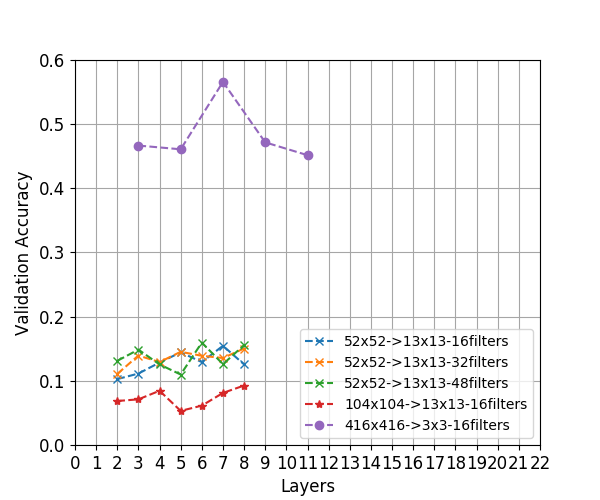
\includegraphics[width=0.8\textwidth]{cropnet}
%	\caption{Validation Accuracy on a set of 1000 %images. The legend shows input resolution followed by %output resolution and the number of filters per layer.}
%\end{figure}


\subsection{Second Stage}

From each image of the dataset a 1:1 crop around the largest bounding box is selected and resized (average pooling) to a 52x52. Different versions of gatenet are applied on that crop. Precision and recall are evaluated for different IoU thresholds to se how accurate the bounding boxes are.

\section{Conclusion}
\begin{itemize}
	\item
\end{itemize}

\section{Next Steps}
\begin{itemize}
	\item Investigate effect of quantization on performance and speed
	\item Investigate effect of depthwise separable convolutions on performance and speed
	
\end{itemize}

\newpage
\appendix


%----------------------------------------------------------------------------------------
\bibliographystyle{abbrv}

\bibliography{literature}

%----------------------------------------------------------------------------------------


\end{document}\grid
